\documentclass[12pt]{article}


\usepackage{graphicx} % Required for inserting images
\usepackage{subcaption}
\usepackage{amsthm}
\usepackage{amsfonts} % or \usepackage{amssymb}
\usepackage{algpseudocode}
\usepackage{algorithm}
\usepackage{float}
\usepackage{amsmath}
\usepackage{verbatim}
\usepackage{xcolor}
\usepackage{tikz}
\usepackage{titlesec}
\usepackage{ebgaramond}

\usepackage[utf8]{inputenc}
\usepackage[english]{babel}
\usepackage{csquotes}  % Recommended for biblatex
\usepackage[backend=biber, style=numeric]{biblatex}
\addbibresource{references.bib} % Make sure your .bib file is correctly named and located

\usepackage{hyperref}
\usepackage{etoolbox}  % Ensure this package is included

% Define the \citeauthorplus command
\newrobustcmd{\citeauthorplus}[1]{\citeauthor{#1} [\citenum{#1}]}


\usetikzlibrary{arrows.meta, positioning, automata}

\theoremstyle{definition}
\newtheorem{definition}{Definition}[section]
\newtheorem{theorem}{Theorem}[section]
\newtheorem{lemma}{Lemma}[section]
\newtheorem{remark}{Remark}[section]
\newtheorem{example}{Example}[section]
\newtheorem{reminder}{Reminder}[section]
\newtheorem{assumption}{Assumption}[section]
\newtheorem{note}{Note}[section]
\newtheorem{proposition}{Proposition}[section]

\algrenewcommand\algorithmicrequire{\textbf{Input:}}
\algrenewcommand\algorithmicensure{\textbf{Output:}}

\DeclareMathOperator*{\argmin}{arg\,min}
\DeclareMathOperator*{\argmax}{arg\,max}

% \newcommand{\citeauthorplus}[1]{\citeauthor{#1} [\citenum{#1}]}

\setlength{\parindent}{0pt}
\setlength{\parskip}{0.5em} % Adjust '1em' to your preference

\titleclass{\subsubsubsection}{straight}[\subsection]

\titleformat{\subsubsubsection}
  {\normalfont\normalsize\bfseries}{\thesubsubsubsection}{1em}{}
\titlespacing*{\subsubsubsection}
{0pt}{3.25ex plus 1ex minus .2ex}{1.5ex plus .2ex}

\setcounter{secnumdepth}{4}
\newcounter{subsubsubsection}[subsubsection]
\renewcommand\thesubsubsubsection{\thesubsubsection.\arabic{subsubsubsection}}

\usepackage[a4paper]{geometry}
\geometry{
 left=15mm,   % Sets the left margin
 right=15mm,  % Sets the right margin
 top=15mm,    % Sets the top margin
 bottom=15mm  % Sets the bottom margin
}

\usepackage{titlesec}

% Set spacing for section/subsection/subsubsection if needed
\titleformat{\section}
  {\normalfont\Large\bfseries}{\thesection}{1em}{}
\titleformat{\subsection}
  {\normalfont\large\bfseries}{\thesubsection}{1em}{}
\titleformat{\subsubsection}
  {\normalfont\normalsize\bfseries}{\thesubsubsection}{1em}{}

% Set the spacing for paragraph
\titlespacing{\paragraph}
  {0pt}{0.5em}{0.1em} % left margin, space before, space after

% Customize this as needed for your document




\title{Time Series Analysis - Final Project \\ \Large Apple Stock Price Prediction}
\author{Gur Keinan 213635899, Technion \and Idan Pipano 213495260, Technion}
\date{May 9th, 2024}


\begin{document}
\pagestyle{empty} % No headers or footers (including page numbers)
\maketitle
\thispagestyle{empty} % Ensures that no page number appears on the title page

\tableofcontents

\newpage  

\setcounter{page}{1} % reset the page counter
\pagestyle{plain} % start showing page numbers
\pagenumbering{arabic} % sets the page numbering style to Arabic numerals

\section{Introduction}

\subsection{The selected dataset}
We used the Apple stock price dataset from Yahoo Finance, available at \url{https://finance.yahoo.com/quote/AAPL/history?p=AAPL}.
The dataset contains the daily stock prices of Apple Inc. from 1980 to 2021.  
We choose to focus on the data from January 1st, 2019 to January 1st, 2024, intentionally including the coronavirus pandemic period. 
The data is a daily time series, however, it is not continuous, as the market is closed on weekend and holidays. We won't pay it much attention and remove the timestamps of the days the market is closed because we only consider the days when the market is open as observations.
It has 1258 records, one for each day in the period, excluding the days the market is closed.
Each record consists of the following columns: 
\begin{enumerate}
  \item \textbf{Date:} The date of the record.
  \item \textbf{Open:} The price of the stock at the opening of the trading day.
  \item \textbf{High:} The highest price of the stock during the trading day.
  \item \textbf{Low:} The lowest price of the stock during the trading day.
  \item \textbf{Close:} The price of the stock at the closing of the trading day.
  \item \textbf{Adj Close:} The adjusted closing price of the stock. The adjusted closing price takes into account factors such as dividends, stock splits, and other corporate actions that may affect the stock price. It provides a more accurate representation of the stock's value compared to the closing price. The adjusted closing price is commonly used in financial analysis and time series analysis to account for these adjustments and ensure consistency in data analysis.
  \item \textbf{Volume:} The number of shares traded during the trading day. It indicates the level of activity in the stock and can provide insights into market sentiment and investor behavior.
\end{enumerate}


\subsection{Domain background}
Stock price prediction is a challenging and important problem in finance and investment. 
Investors and traders rely on accurate stock price forecasts to make informed decisions about buying, selling, or holding stocks. 
Time series analysis is a powerful tool for modeling and predicting stock prices based on historical data. 
By analyzing past stock price movements and patterns, time series models can identify trends, seasonality, and other patterns that can help predict future stock prices.

There are several approaches to stock price prediction using time series analysis. 
Some of the popular methods include autoregressive integrated moving average (ARIMA) models, exponential smoothing, and the Prophet model, which is particularly well-suited for handling daily data that exhibits multiple seasonalities. 
Following these, machine learning algorithms such as random forests and deep learning models like recurrent neural networks (RNNs) and long short-term memory (LSTM) networks, are commonly employed. 
Additionally, Kalman filters represent another sophisticated approach that uses a series of measurements observed over time, containing statistical noise and other inaccuracies, and produces estimates of unknown variables that tend to be more precise than those based on a single measurement alone.

These models can capture complex patterns in stock price data and make accurate predictions based on historical trends and patterns.
In addition to historical stock price data, external factors such as economic indicators, news sentiment, and market sentiment can also impact stock prices. By incorporating these external factors into the analysis, time series models can improve the accuracy of stock price predictions and provide more reliable forecasts for investors and traders.

\subsection{Data exploration and visualization}
In this subsection we will analyze the dataset, and present some visualizations of the data.

\begin{minipage}{0.5\textwidth} % Adjust the width to fit your needs
  \fbox{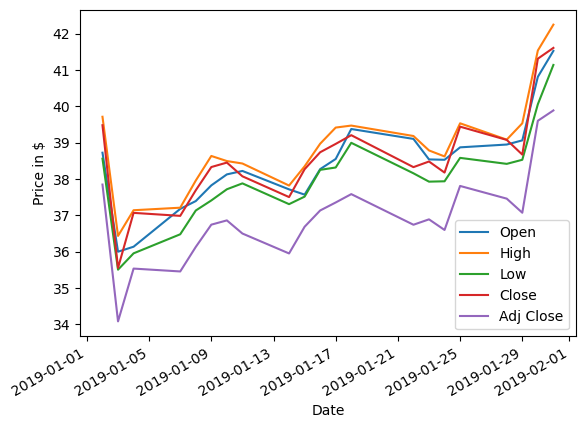
\includegraphics[width=\linewidth]{Images/all_columns_graph.png}}
\end{minipage}%
\hfill % Optional: Adds horizontal space between the minipages
\begin{minipage}{0.45\textwidth} % Adjust the width accordingly
  In this graph we can see the stock price data of Apple at January 2019. It includes the open, high, low, close, and adjusted close prices. 
  It's not unusual for the adjusted close price to be lower than the close price, as it accounts for factors such as dividends and stock splits that may affect the stock price. 
  We can see similar trends and seasonality in all the prices, as expected based on their similar nature. 
  We show this graph to give a general idea of the data we are working with, and to give a closer look at the adjusted close price, which is our target variable for forecasting.
\end{minipage}

\begin{minipage}{0.5\textwidth} % Adjust the width to fit your needs
  \fbox{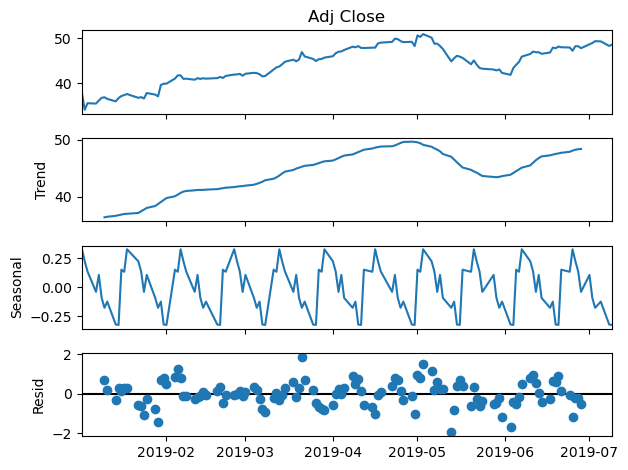
\includegraphics[width=\linewidth]{Images/seasonal_decompose.png}}
\end{minipage}%
\hfill % Optional: Adds horizontal space between the minipages
\begin{minipage}{0.45\textwidth} % Adjust the width accordingly
  In this graph we show the seasonal and trend components of the adjusted close price of Apple stock between January 2019 and June 2019. 
  We took a subset of the data to better visualize the seasonal patterns, they are consistent through the whole dataset.
  We can clearly see repeating patterns during this period, indicating the presence of seasonality in the data.
  The trend component doesn't persist for long periods, which is expected in stock price data that is known to be volatile and subject to sudden changes.
  We can see that the residuals are nicely centered around \(0\) and have relatively similar spread, indicating that the decomposition captures most of the patterns in the data. 
  This also happens in the whole dataset, and we show this graph to give a general idea of the seasonality and trend in the data.
\end{minipage}

\subsection{Problem statement}
In this project we will focus on the two following tasks:
\begin{itemize}
  \item Develop time series models to accurately forecast the adjusted closing price of Apple stock in an online learning setting, where the model is updated with new data daily. 
  We prefer this setting rather than training the model once on the whole dataset, as it is more realistic for real-life applications where new data is continuously available. 
  We will focus on classical time series models, such as autoregressive integrated moving average (ARIMA), Prophet, and Kalman filter, as well as machine learning models, including long short-term memory (LSTM) networks. 
  The performance of these models will be evaluated to asses their accuracy and reliability in predicting stock prices.
  \item Investigate the impact of external factors such as economic indicators on stock price predictions. 
  We will evaluate the models with and without the inclusion of external data to determine whether incorporating additional information improves the accuracy of the forecasts.
\end{itemize}

\subsection{Project structure}
The rest of the paper is organized as follows:
\begin{itemize}
  \item \textbf{Section 2} - Methodology: We will describe the models used for fitting and forecasting the stock prices, as well as the integration of external data.
  \item \textbf{Section 3} - Results and Discussion: We will present the results of the models, compare their performance, and analyze the impact of external data on stock price predictions.
  \item \textbf{Section 4} - Conclusions and future work: We will summarize the key findings of the project and discuss potential future directions for research and analysis.
\end{itemize}


\section{Methodology}

First we describe our approach for fitting and evaluating the models.
80\% of the data will be used for training the models, while the remaining 20\% will be used for testing and evaluating the predictions (this split roughly translates to 4 years of training data and 1 year of testing data).
The training and testing processes under the online settings will be performed as follows:

\begin{algorithm}[H]
  \caption{Online learning process}
  \begin{algorithmic}
    \Require{Training data $\{ X_t, y_t \}_{t \in Train}$, Testing data $\{ X_t, y_t \}_{t \in Test}$}
    \Ensure{Predictions $\hat{y}_t$ for each $t \in Test$}
    \State \textit{Fit} the model on the training data $\{ X_t, y_t \}_{t \in Train}$  \Comment{Can be done only once, can be more time-consuming}
    \For{each $t \in Test$}
      \State \textit{Forecast} the next day's price $\hat{y}_t$  \Comment{Can be easily generalized to multiple days ahead}
      \State \textit{Update} the model with the new data $X_t, y_t$  \Comment{Efficient and fast updating}
    \EndFor
  \end{algorithmic}
  \label{alg: online learning process}
\end{algorithm}

The evaluation will be performed using 2 methods. 
The first is measuring the error of the predictions using the Root Mean Squared Error (RMSE) score. 
This is a widely used measure for evaluating the performance of time series models which is known for penalizing large errors and for being sensitive to outliers. 
Both of those properties are important for investors, as they want to avoid large losses and are sensitive to extreme events.
For clarity, bellow is a formal definition of the RMSE score on the test data:
\[
  RMSE = \sqrt{\frac{1}{|Test|} \sum_{t \in Test} (y_t - \hat{y}_t)^2}
\]

The second method is visualizing the predictions of the models and comparing them to the actual values.
Although seems more naive, this method is important for understanding the behavior of the models and for getting a better intuition about the predictions.
As to be seen throughout the project, the visualizations can give insights that the RMSE score doesn't reflect, and therefore are important for the evaluation process.

\subsection{Used models for forecasting}
\paragraph{SARIMA}
The Seasonal Autoregressive Integrated Moving Average (SARIMA) model,
the foundation to which were laid by \citeauthor{box2015time} in \cite{box2015time},
is employed to capture both non-seasonal and seasonal trends and cycles in the stock price data. 
It consists of three main components: the autoregressive (AR) component, the differencing (I) component, and the moving average (MA) component.
The parameters of the SARIMA model are denoted as $(p, d, q)$ for the non-seasonal part and $(P, D, Q, S)$ for the seasonal part, where $p$, $d$, and $q$ are the order of the AR, I, and MA components, respectively, and $P$, $D$, $Q$, and $S$ are the seasonal parameters.
The training of the model involves optimizing these parameters to minimize the Akaike Information Criterion (AIC) on the training data. 
The AIC, intoduced in \cite{akaike1974new}, is a measure of the relative quality of a statistical model for a given dataset which 
takes into account both the goodness of fit and the complexity of the model.
Our implementation makes use of python's \textit{pmdarima} library \textit{auto\_fit} function which enables automatic fit of the model, and the SARIMAX library to implement the SARIMA model - it includes the \textit{fit}, \textit{forecast}, and \textit{append} functions to train the model, make predictions, and update the model with new data, respectively.
The use of the \textit{append} function is crucial for the online learning setting, as it allows to update the model with new data without retraining the entire model - the model's parameters are learned during training and fixed during testing.

\paragraph{Prophet}
Prophet, developed by Facebook and presented in \cite{taylor2018forecasting}, is utilized for its robust handling of daily data with multiple seasonalities and the inclusion of holiday effects. 
It fits nonlinear trends with yearly, weekly, and daily seasonality.
The model parameters include the changepoint prior scale, seasonality prior scale, and holidays prior scale, which control the flexibility of the model in capturing trends and seasonal patterns.
We tune these parameters to optimize the model's performance on the training data.
In Prophet's framework there isn't a built-in function for online learning and updating.
Our solution for this is to use an "warm up" option, where in each iteration one saves the fitted model and then uses it to get an advanced start for the next training given the new data.
It turns out to be quite efficient and gives good results, as the model is already well fitted to the data and only needs to adjust to one more timestamp.
This method of online training and forecasting was suggested by the prophet developers, for more information see \url{https://github.com/facebook/prophet/blob/main/notebooks/additional_topics.ipynb}.

\paragraph{Kalman filter}
The Kalman filter, first presented in \cite{kalman1960new}, is applied to estimate hidden states in the stock price data dynamically, allowing for real-time updates and predictions. 
It is particularly useful for adjusting forecasts based on new daily inputs.
The model parameters include the state transition matrix, observation matrix, process noise covariance, and measurement noise covariance, which are optimized to improve the accuracy of the predictions.
Kalman filter is already well suited for online learning, as it is designed to update the model with new data and provide more accurate estimates of the hidden states.
The classic Kalman filter method includes predicting the next state and updating the model with the new data.
Therefore, we introduce a slight change to the method to fit the online learning setting - in each iteration the prediction is made without updating the model, and then the model is updated with the new data.
We point out that Kalman filter has unfair advantage over the other models, as it is designed to fit himself to the new data automatically and not necessarily stay true to the parameters it learned during training.
Because its update is done in an efficient way, we consider it to be a good model for online learning and use it anyway, but one should take this point into consideration when comparing the models.
Our implementation make use of python's \textit{pykalman} library for implementing the Kalman filter model and the \textit{filter} and \textit{update} functions to update the model with new data and make predictions.

\paragraph{Long Short-Term Memory (LSTM)}
Introduced by \citeauthor{hochreiter1997long} in \cite{hochreiter1997long}, the LSTM architecture is a type of recurrent neural network (RNN) that is well-suited for capturing long-term non-linear dependencies in sequential data.
The classic LSTM architecture includes multiple LSTM layers with dropout regularization to prevent overfitting. 
Each LSTM layer consists of a cell state and hidden state that represent the long-term and short-term memory of the model, respectively.
LSTM uses designated gates in order to preserve or discard information at each time step, allowing it to capture long-term dependencies in the data.
Those gates are the forget gate (decides what information to throw away from the cell state), the input gate (decides what new information to store in the cell state), and the output gate (decides what to output based on the cell state).
As a preprocessing step, the data is normalized to improve the convergence of the model during training.
Then, using a sliding window approach, the data is transformed into sequences of input features and target variables.
Each input consists of \textit{lookback} days of stock prices, and the target variable is the stock price of the next day.
The splitting to train and test data is done in the same way as the other models, and the model is trained on the train data and evaluated on the test data.
The learned parameters are fixed during testing.
The online updating of the model is done by providing to the model the real data as observations in the test data, and not the predictions of the model.
Off course, it's done carefully to avoid data leakage and only use the data that was available at the time of the prediction.
Our implementation is done using the TensorFlow and Keras libraries in Python, and the architecture of the model is presented in Appendix \ref{app: LSTM architecture}.
After experimenting with multiple architectures, we found that a simple LSTM model without many layers and dropout regularization gives the best results, and therefore we used this architecture for the model. 

\subsection{Integration of external data}
For starters, we will use the rest of the columns of the Apple stock dataset as external data.
In addition, data of the stock ICE US Dollar Index will be added. This index is a measure of the value of the United States dollar relative to a basket of foreign currencies. 
It is a weighted geometric mean of the dollar's value compared to a group of other major currencies, including the euro, Japanese yen, British pound, Canadian dollar, Swedish krona, and Swiss franc. 
The index is used to track the dollar's performance against other currencies and is a key indicator of the dollar's strength in the global economy. 
The data can be found at \url{https://finance.yahoo.com/quote/DX-Y.NYB/}.
It has the same recorded dates as the Apple stock dataset, and we used it as an external factor that might influence the stock price of Apple. 
We expect the external index data to be informative and to improve the accuracy of the forecasts, as the stock price of Apple is influenced by the global economy and the value of the dollar in the global market.

We modified 3 of our models to incorporate the external data - SARIMA, Kalman filter, and LSTM.
Bellow is a short description of the necessary changes we made to the models to do so.
\begin{itemize}
  \item SARIMA - the external data was added as an exogenous variable to the model, and used the \textit{SARIMAX} library and its built-in methods to implement the model with the external data. 
  The forecasting was done carefully to prevent data leakage - only the available data in the time of the prediction was used.
  For doing so, when forecasting, we passed the last available exogenous data to the model, although the standard way of using this functionality is to pass the future exogenous data to the model.
  \item Kalman filter - the external data was integrated as an additional observation to the model, and the \textit{filter} and \textit{update} functions were used to update the model with the new data. 
  Kalman filter is easily adjustable to the the multivariate settings, as it is designed to handle multiple observations and states.
  \item LSTM - the external data was integrated as additional features to the model - each input to the model now consists of the stock prices of the last \textit{lookback} days and the external data of the same days. 
  The same architecture as before was used, but with larger input size and more features.
  The LSTM model is well suited for this task, as it can capture complex relationships between the stock price and the external data.
\end{itemize}

Our goal will be to examine the effect of the external data on the predictions of the models, and to see if it improves the accuracy of the forecasts.

\subsection{Predicting several days ahead}
Success in the stock market often involves predicting the market prices several days into the future, not just one. 
Extending predictions to a longer horizon increases their utility but also their difficulty due to the increased uncertainty and the impact of external factors.
We took it upon ourself to expand our goal to include the stock price prediction for several days ahead.

For clarity, we describe the process of predicting \(D\) days ahead in the online learning setting in Algorithm \ref{alg: D days ahead}, as there are many ways to do so and we want to make sure the reader understands our approach.

\begin{algorithm}[H]
  \caption{Online learning process - predicting \(D\) days ahead}
  \begin{algorithmic}
    \Require{Data $\{ X_t, y_t \}_{t=1}^{N}$, first test prediction index $t_0$, depth $D$}
    \Ensure{Predictions $\hat{y}_t = f( \{ X_k, y_k \}_{k=1}^{t-D} )$ for each $t_0 \leq k \leq N$}
    \State \textit{Fit} the model on the training data $\{ X_t, y_t \}_{1 \leq t \leq t_0 - D}$  \Comment{Can be done only once, can be more time-consuming}
    \For{each $t \in \{t_0, \dots, N\}$}
      \State \textit{Forecast} $\hat{y}_t$ using $\{ X_k, y_k \}_{k=1}^{t-D}$
      \State \textit{Update} the model with $ X_{t-D+1}, y_{t-D+1} $  \Comment{Efficient and fast updating}
    \EndFor
  \end{algorithmic}
  \label{alg: D days ahead}
\end{algorithm}

Notice that for $D=1$ this algorithm is the same as Algorithn \ref{alg: online learning process}.
The training and forecasting in SARIMA and prophet were done in the same way as before with slight adjustments.
The Kalman filter was slightly more problematic as it didn't have a built-in function to predict several days ahead. 
We implemented it by saving its parameters in the beginning of each iteration, updating the states without observations several times until we reached the desired depth, and only then updating the saved parameters with the new data.
The training of the LSTM was done by simply changing the target variable to be the price of the day in the desired depth.
The evaluation methods remained the same.

\section{Results and Discussion}

\subsection{Models results and visualizations}
The following figure provides a visual comparison,
as well as a quantitative comparison in terms of RMSE scores,
of the test predictions of the different models when predicting one day ahead.

\begin{figure}[H]
  \centering
  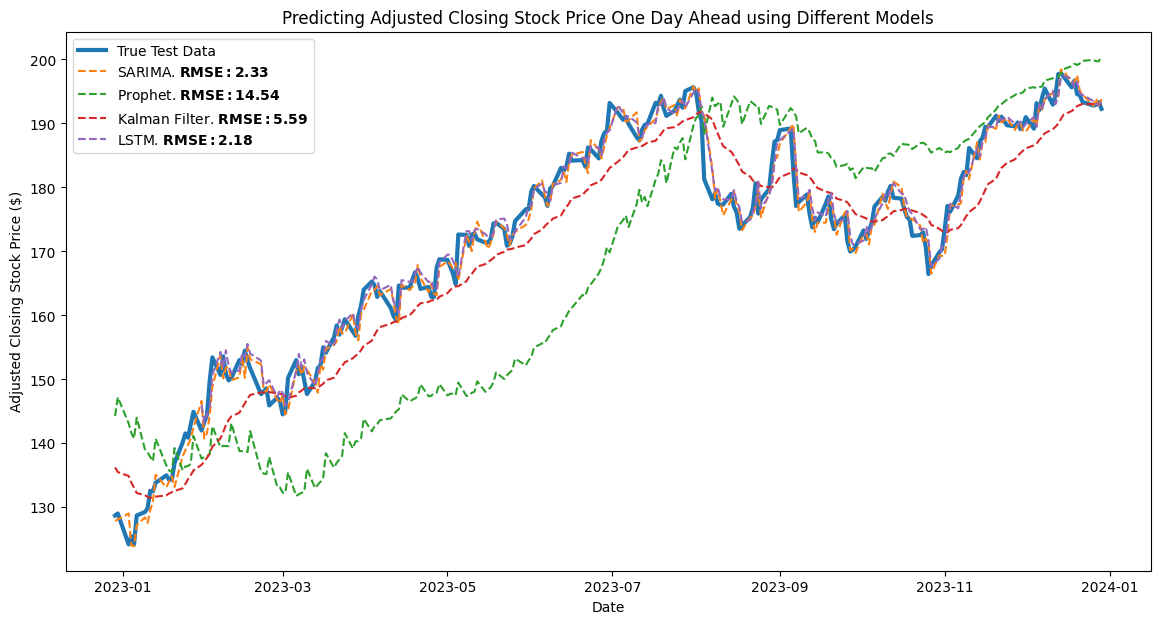
\includegraphics[width=0.95\textwidth]{Images/one day ahead compilation.png}
  \caption{one day ahead RMSE and forecast comparison of the models}
\end{figure}

The continuous blue line is the real stock price. 
Very close to it are the dashed orange and purple lines, which represent the predictions of the SARIMA and LSTM models, respectively. 
The dashed red line is the prediction of the Kalman filter, and the dashed green line is the prediction of the Prophet model.
We can see that the LSTM and SARIMA models are the best performing models, with the lowest RMSE scores and (suspiciously) accurate predictions.
The LSTM performed a bit better than the SARIMA model, but the difference is negligible.
After them is the Kalman filter, which gives a more round and robust view of the stock, without the sharp changes in trend.
One can see it following the general trend of the stock but not predicting the sharp changes in the stock price like the former models.
Last in performance is the Prophet model, which is the least accurate of all the models. 
Our guess about the reason for its downfall is that Prophet tries to capture the seasonality and the overall trend in the data, and the stock prices are very unstable and sensitive to foreign influence which happens daily, and therefore it is not well suited for our purpose of online learning. 

\subsection{Discussion}

\paragraph{Why does SARIMA pperform so well compared to Prophet?} 
SARIMA's superior performance in this project compared to Prophet can be explained by the uncertain nature of the stock market.
We suspect that the stock market is too volatile and sensitive to external factors for Prophet to capture its trends and seasonality.
On the other hand, the AR aspect of SARIMA allows it to capture the immediate past trends and adjust to the sudden changes in the stock price.
Therefore, it can be more accurate in predicting the stock price in the short term, and especially in the online learning setting where the model is updated with new data daily.
Although Prophet consists of sophisticated components that can capture multiple seasonalities and holiday effects, it may not be well-suited for predicting the stock market, which is influenced by numerous unpredictable external factors.

\paragraph{Suspicious Success of SARIMA and LSTM}
When looking at the scale of the data, one gets suspicious about the low RMSE scores of the SARIMA and LSTM models - the adjusted close prices range from 120\$ to almost 200\$ in the dataset, and the RMSE scores are less than 3\$.
We looked more closely at the results and discovered an interesting finding - both models always predict a slightly shifted version of the last known value at the time of prediction.
This means that the models learned that the best way to minimize the RMSE is to predict the same value as the last known value, just shifted by one day.
It raised the following question - what will be the RMSE if we naively return the last known value as the prediction? We found out that \textbf{this naive method outperformed all the models}. 
This is not encouraging - predicting the last known value is not informative at all and won't help in real-life scenarios.

\paragraph{Kalman filter advantages}
The Kalman filter, on the other hand, perform slightly worse than the SARIMA and LSTM models, but it has some advantages over them.
When looking at the predictions it gives, one can see that it is more stable and won't just predict the last known value.
We think that this is because of its original purpose, the Kalman filter is designed to predict the underlying structure of the data, and not the data itself.
Therefore it can reveal the true trend of the stock, and be useful for stock price prediction.

\subsection{Analyzing external data impact}
Bellow are the results of the models with the external data added to them.

\begin{figure}[H]
  \centering
  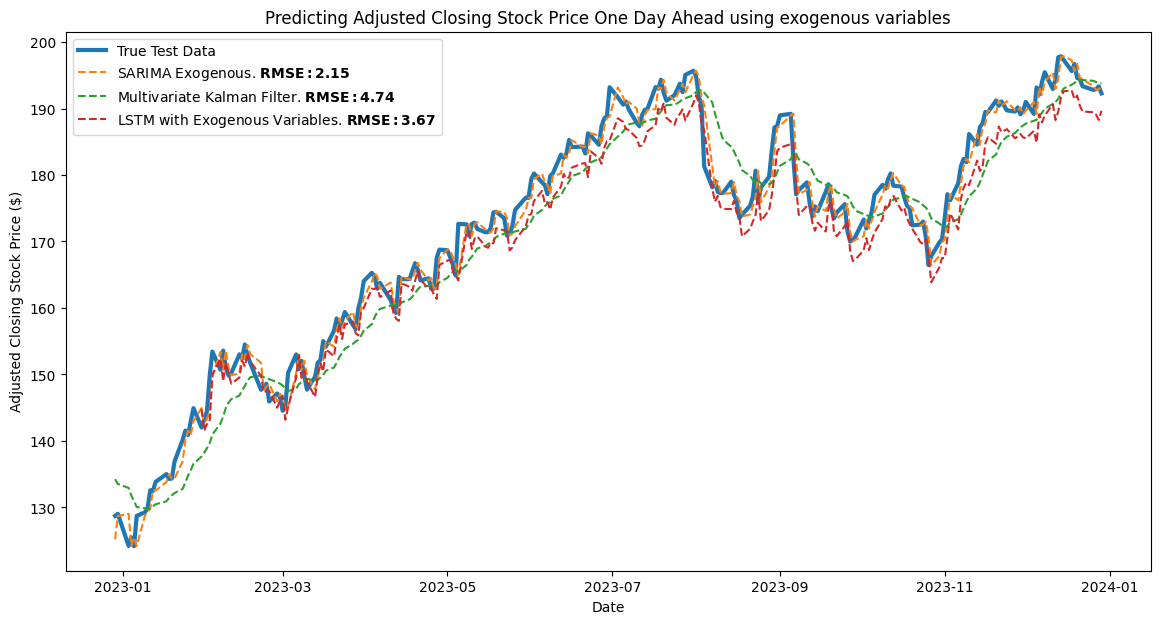
\includegraphics[width=0.95\textwidth]{Images/one day ahead exogenous compilation.png}
  \caption{RMSE and forecast comparison of the models with external data}
\end{figure}
The continuous blue line is the real stock price, and the dashed lines are the predictions of the models.
Once again, the SARIMA and LSTM models are the best performing models.
The SARIMA model was the least affected by the external data, as it already captures the seasonality and trend in the data, and the external data didn't add much to it.
On the other hand, the LSTM model performance slightly declined when incorporating external data, as it was probably harder for the model to capture the relationships between the stock price and the external data.
We suspect that further hyper-parameter tuning and architecture modifications can improve the LSTM's performance, but not significantly, because it already achieved a very low RMSE score without the external data.
In addition, expanding the training data to include more previous days might be beneficial for the LSTM model.
We didn't do it because we wanted to keep the training data consistent for all the models, but we suspect that it would affect the LSTM the most.
The Kalman filter enjoyed the external data, as it gave a more robust and stable prediction. 
Our explanation for this improvement is that the rest of the columns of the stock affected it the most and helped to bound it and keep it from deviating too much.
Other experiments we made by removing some of the columns of the stock data support this conjecture.


\subsection{Predicting several days ahead}
Bellow is visualization of the prediction of the different models when predicting 1, 5 and 10 days ahead.

\begin{figure}[H]
  \centering
  
  % First row, first image
  \begin{subfigure}[b]{0.49\textwidth}
      \centering
      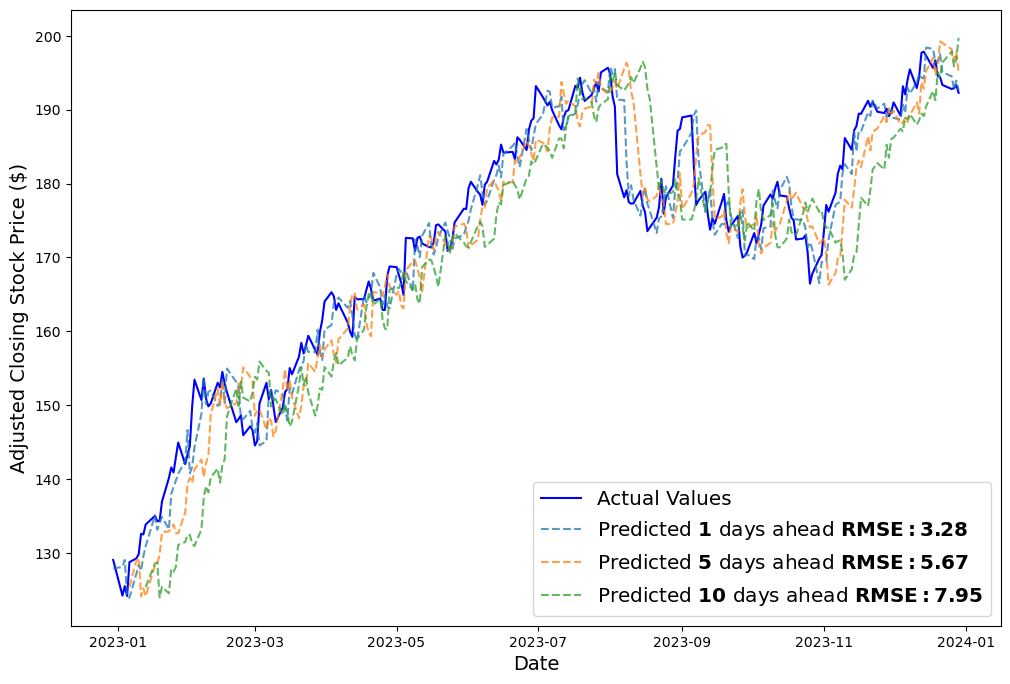
\includegraphics[width=\textwidth]{Images/SARIMA multiple days ahead.png}
      \caption{Predicting multiple days ahead with SARIMA}
      \label{fig:image1}
  \end{subfigure}
  \hfill % Space between the images
  % First row, second image
  \begin{subfigure}[b]{0.49\textwidth}
      \centering
      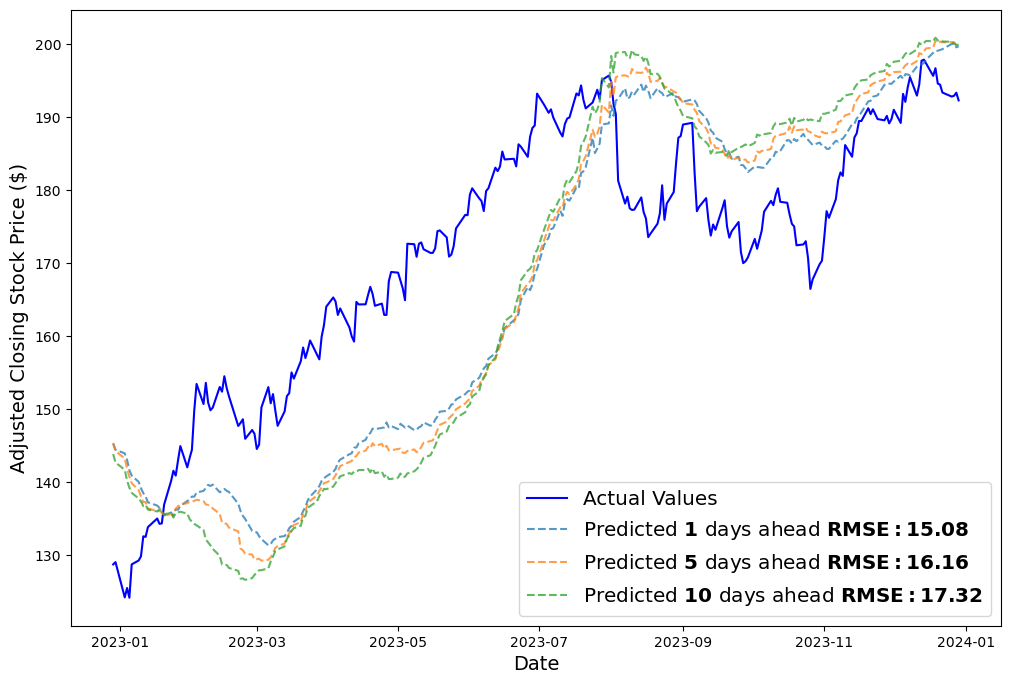
\includegraphics[width=\textwidth]{Images/Prophet multiple days ahead.png}
      \caption{Predicting multiple days ahead with Prophet}
      \label{fig:image2}
  \end{subfigure}
  
  % Second row, first image
  \begin{subfigure}[b]{0.49\textwidth}
      \centering
      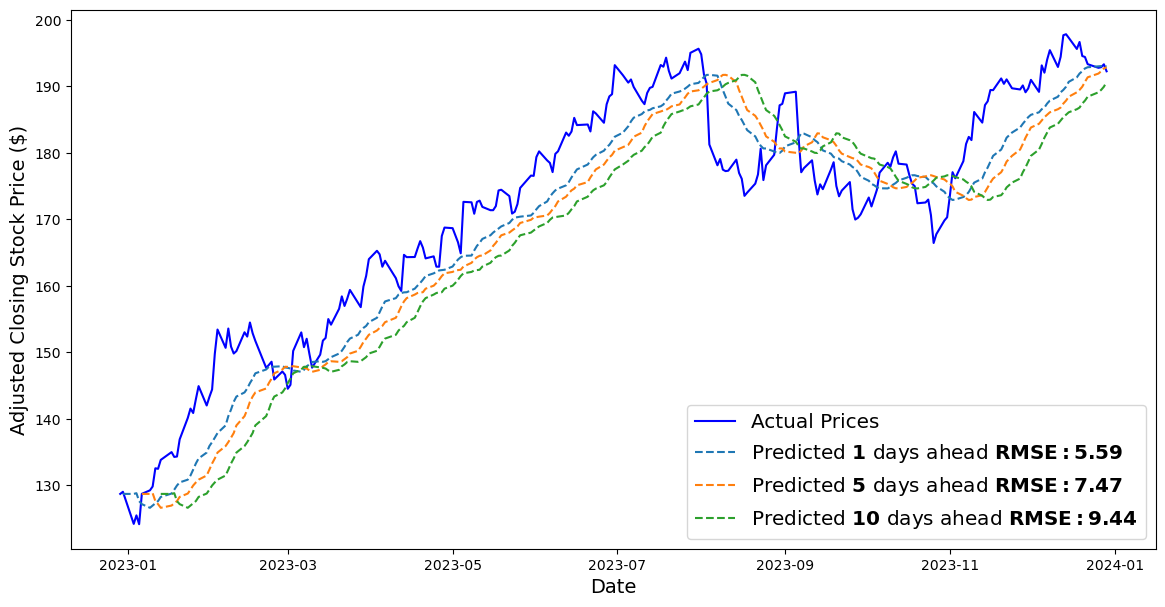
\includegraphics[width=\textwidth]{Images/Kalman filters multiple days ahead.png}
      \caption{Predicting multiple days ahead with Kalman filter}
      \label{fig:image3}
  \end{subfigure}
  \hfill % Space between the images
  % Second row, second image
  \begin{subfigure}[b]{0.49\textwidth}
      \centering
      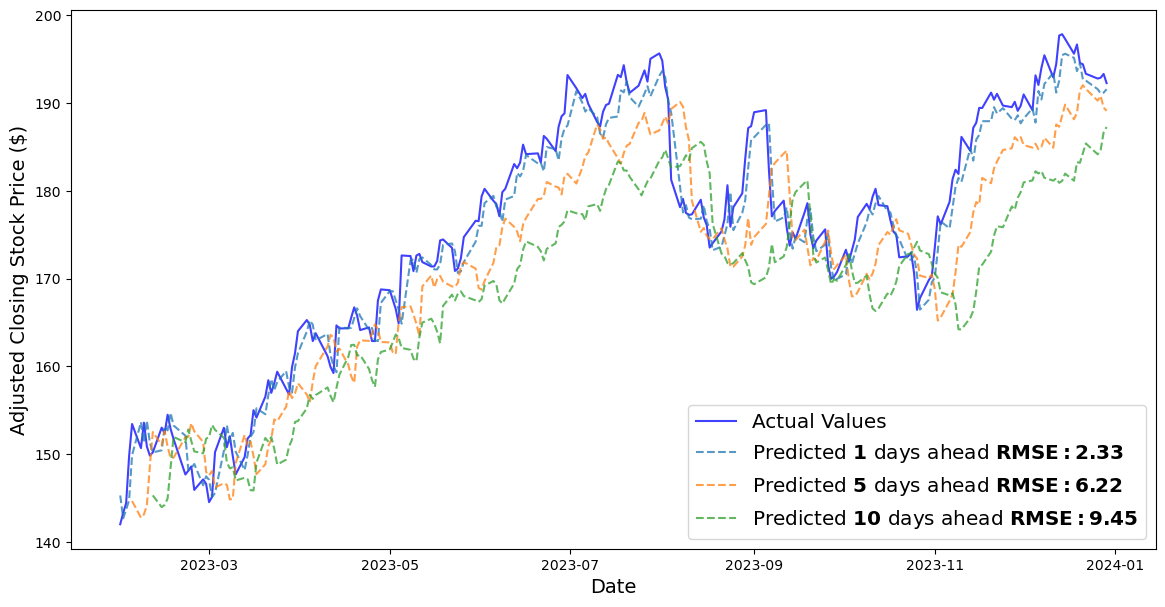
\includegraphics[width=\textwidth]{Images/LSTM multiple days ahead.png}
      \caption{Predicting multiple days ahead with LSTM}
      \label{fig:image4}
  \end{subfigure}
  
  \caption{Comparison of the models when predicting multiple days ahead}
  \end{figure}

We can see that the SARIMA and LSTM models achieve the best results,
while the performance of Kalman filter is relatively good and Prophet's performance is the worst.

One can notice an interesting phenomenon which happens for all of the models except for, surprisingly, the Prophet model. 
When looking beyond the low RMSE scores, one can see that those models predict the same shifted "template", no matter how many days ahead we entered as input. 
This means that instead of trying to predict the values according to trend or seasonality, the models learned that for achieving low RMSE they need to try to predict the same values as the input, just shifted by the number of days ahead.
In the contrary, the Prophet model doesn't show this behavior, and one can see that its predictions converges at some timestamp to be the same, no matter the depth of the prediction.
This is the kind of behavior we want from our models - consistency and stability in the predictions.
Still, we will prefer the other models because the Prophet performance is much worse than the other models and is too weak to be considered as a good model for stock price prediction.

The analysis of all of the models yield the same conclusion - predicting far into the future in the stock market is hard, as the market is very sensitive to external factors and is very volatile.
The trends it presents are unexpected and can change rapidly, and therefore it is hard, if not impossible, to predict the stock price far into the future.
On the other hand, we saw that we can achieve good results when predicting one day ahead, but this is because those models learned to predict the same value as the input, just shifted by one day, which is not informative at all.

\section{Conclusions and Future Work}

\paragraph{Summary of Findings}
Our analysis of various time series models for predicting Apple stock prices reveals that the most simplistic model, which predicts tomorrow's stock price as today's closing price, often outperforms more complex models like SARIMA, Prophet, Kalman filter, and LSTM. This observation underscores the inherent difficulty in predicting stock market movements, which are influenced by numerous unpredictable external factors.

\paragraph{The Efficient Market Hypothesis Revisited}
The Efficient Market Hypothesis (EMH), proposed in \cite{fama1970efficient} and explained in 
a more accessible manner at \url{https://www.investopedia.com/terms/e/efficientmarkethypothesis.asp},
posits that stock prices reflect all available information and adjust rapidly to new information, making it impossible to consistently achieve returns that exceed average market returns without assuming higher risks. Our findings lend support to EMH, as even sophisticated models with access to historical data and external variables could not outperform a naive baseline. This suggests that the stock market efficiently incorporates information into prices, leaving little room for predictive models to exploit any informational advantages.

\paragraph{Performance of Time Series Models}
\begin{itemize}
    \item \textbf{SARIMA and LSTM} performed slightly better in short-term predictions, largely because they effectively captured the immediate past price trends. However, their success diminishes with the increase in the prediction horizon, highlighting their limitations in dealing with the stock's volatility and external shocks.
    \item \textbf{Kalman Filter} provided a more robust performance by adapting to new data points and offering a stable prediction pathway. Its ability to dynamically adjust to new information makes it a valuable tool, particularly for applications requiring real-time data assimilation. In addition we saw its advantages when we closely analyzed the predictions and saw that it doesn't predict the last known value, but rather the underlying structure of the data.
    \item \textbf{Prophet} struggled due to its focus on capturing broad trends and seasonality, which are less pronounced in the highly volatile stock price movements.
\end{itemize}

\paragraph{Impact of External Data}
The inclusion of external data, such as the ICE US Dollar Index, had a mixed impact on the models. 
While the SARIMA model remained largely unaffected, the LSTM model's performance slightly declined with the addition of external data. 
The Kalman filter benefited from the external data, providing a more stable and robust prediction pathway. 
These results suggest that the impact of external data on stock price predictions can vary depending on the model's architecture and the nature of the data.
We hypothesis that further experiments with different external data sources and feature engineering could improve the models' performance and provide more accurate forecasts, especially for the more complicated models as the Kalman filter and LSTM which may find a better use of the external data for modeling the stock price.

\paragraph{Implications for Investors}
For investors, our study suggests that relying on sophisticated predictive models may not necessarily provide an edge over a simple strategy based on recent price trends. 
This finding emphasizes the importance of risk management and diversification over trying to predict future stock prices.

\paragraph{Future Work}
Further research could explore the integration of more diverse datasets, including high-frequency trading data, social media sentiment (e.g., people's sentiment about Apple), and macroeconomic indicators, to assess whether these can enhance the predictive power of models. 
Additionally, machine learning techniques that focus on pattern recognition and anomaly detection could be used to identify short-lived trading opportunities that are not captured by traditional models.
Finally, it's worth exploring a premature event inclusion in the models, as the stock market is very sensitive to external factors and can change rapidly due to unexpected events. If one has access to such future events data (e.g. "Apple will release it's state of the art macbook in a week"), it can be very beneficial for the models and improve their performance.

\paragraph{Final Thoughts}
While time series analysis offers valuable insights into data patterns and potential trends, its application to stock price prediction must be approached with caution. 
The inherent unpredictability of financial markets, governed by external factors and human psychology, makes it a challenging domain for any predictive model. 
Our study reinforces the view that stock market predictions are highly speculative and should be part of a broader strategy that considers financial theory, investor behavior, and market economics.

\printbibliography

\appendix

\section{The LSTM Architecture}\label{app: LSTM architecture}

\begin{figure}[H]
  \centering
  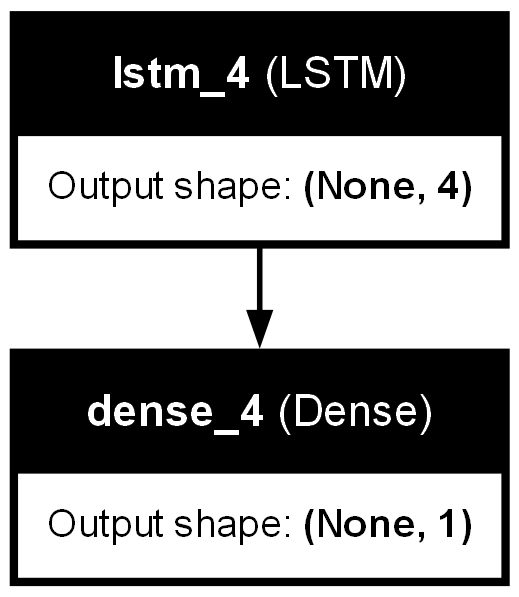
\includegraphics[width=0.35\textwidth]{Images/model_plot.png}
  \caption{LSTM architecture for stock price prediction}
\end{figure}

The architecture consists of an LSTM layer with hidden dimension \(4\), which outputs a vector
of size \(4\) that is then passed through a dense layer with \(1\) output unit.

It is worth mentioning that we 
experimented with a lot of different architectures, different hyper-parameters, and different regularization methods
(dropout, etc.) and found that this simple architecture gives the best results.


\end{document}